%%=============================================================================
%% Proof of Concept
%%=============================================================================

\chapter{\IfLanguageName{dutch}{Proof of Concept}{Proof of Concept}}%
\label{ch:proof-of-concept}

In dit deel van het onderzoek presenteert een proof of concept gericht op de beoordeling van de gekozen navigatiemethoden, die gebruikt kunnen worden voor mensen met een mentale beperking. Het doel van de proof of concept is de efficiëntie, bruikbaarheid en gebruiksvriendelijkheid van deze methoden te onderzoeken aan de hand van een applicatie. De ontwikkeling van deze applicatie en hieruit gehaalde resultaten worden besproken. Als laatste zal er een discussie worden gevoerd, welke navigatietool de meest geschikte is voor de doelgroep.

\section{Ontwikkeling van de applicatie}
\label{sec:ontwikkeling van de applicatie}
In dit onderdeel wordt de opbouw van de applicatie besproken. Hieruit zal duidelijk worden hoe de applicatie opgebouwd is. De code is niet relevant voor het verdere verloop van het onderzoek. Als eerste worden de belangrijkste onderdelen besproken. Een nieuw React Native project wordt aangemaakt aan de hand van Node.js en een terminal. Na het opzetten van dit project, moet er een Mapbox account gecreëerd worden voor een publieke token zodat er gebruik gemaakt kan worden van hun diverse mappen. \newline

In de applicatie is één simpel scherm. Op Figuur \ref{fig:Scherm met een knop om de route op te vragen} is te zien dat er een Mapbox map ingeladen wordt en een invoerveld met een knop. Het proces wordt in gang gezet wanneer op de knop gedrukt wordt en een correct adres is ingegeven. Wanneer een foutief adres wordt ingegeven zal er een foutmelding komen en wordt het proces onderbroken. Bij Figuur \ref{fig:Scherm met knop waar route die opgevraagd is} 

\begin{lstlisting}[caption={Code-voorbeeld van het navigatiescherm}, label=code-voorbeeld navigatiescherm, captionpos=b]
    Mapbox.setAccessToken('MAPBOX_PUBLIC_TOKEN');
    
    const App = () => {
        const [location, setLocation] = useState('');
        const [destination, setDestination] = useState('');
        const [route, setRoute] = useState(null);
        const [errorMsg, setErrorMsg] = useState(null);
        const [isLoading, setIsLoading] = useState(false);
        
        useEffect(() => {
            (async () => {
                let { status } = await Location.requestForegroundPermissionsAsync();
                if (status !== 'granted') {
                    setErrorMsg('Permission to access location was denied');
                    return;
                }
                
                let currentLocation;
                if (Platform.OS === 'OS' && !__DEV__) {
                    currentLocation = await Location.getCurrentPositionAsync({});
                    console.log('Current location:', currentLocation);
                } else {
                    currentLocation = {
                        coords: {
                            longitude: 4.038139399999999,
                            latitude: 50.9318886,
                        },
                    };
                }
                
                if (!currentLocation) {
                    setErrorMsg('Failed to obtain location');
                    return;
                }
                setLocation(currentLocation);
            })();
        }, []);
        
        const getRoute = async () => {
            setIsLoading(true);
            const userLocation = `${location.coords.longitude},${location.coords.latitude}`;
            console.log('User location:', userLocation);
            
            const YOUR_GOOGLE_API_KEY = 'GOOGLE_API_KEY';
            
            const startLong = location.coords.longitude;
            const startLat = location.coords.latitude;
            
            try {
                const destinationCoords = await getCoordinatesFromPlace(destination, YOUR_GOOGLE_API_KEY);
                const endLong = destinationCoords.split(',')[1];
                const endLat = destinationCoords.split(',')[0];
                console.log(endLong, endLat)
                console.log('Destination coordinates:', destinationCoords);
                if(!destinationCoords) {
                    throw new Error('Failed to fetch destination coordinates');
                }
                
                const mapboxUrl = `https://api.mapbox.com/directions/v5/mapbox/walking/${startLong},${startLat};${endLong},${endLat}?alternatives=true&annotations=distance&continue_straight=true&geometries=geojson&overview=full&steps=false&access_token=MAPBOX_PUBLIC_TOKEN`
                console.log('Mapbox Directions API URL:', mapboxUrl);
                const response = await fetch(mapboxUrl);
                const data = await response.json();
                                
                if (data.routes && data.routes.length > 0) {
                    const routeCoordinates = data.routes[0].geometry.coordinates.map(coord => ({ longitude: coord[0], latitude: coord[1] }));
                    // console.log('Route coordinates:', routeCoordinates);
                    setRoute(routeCoordinates);
                } else if (data.coords == 'NoRoute'){
                    throw new Error('No route found');
                } else {
                    throw new Error('Failed to fetch route');
                }
            } catch (error) {
                console.error(error);
                setErrorMsg('Failed to fetch route');
            } finally {
                setIsLoading(false);
            }
        };
        
        const getCoordinatesFromPlace = async (place, apiKey) => {
            const apiUrl = `https://maps.googleapis.com/maps/api/geocode/json?address=${encodeURIComponent(place)}&key=${apiKey}`;
            
            try {
                const response = await fetch(apiUrl);
                
                console.log('Geocoding API response status:', response.status);
                
                if (!response.ok) {
                    throw new Error(`Geocoding API request failed with status ${response.status}`);
                }
                
                const data = await response.json();
                                
                if (data.status === 'OK' && data.results.length > 0) {
                    const result = data.results.find(result => result && result.geometry && result.geometry.location);
                    if (result) {
                        const { lat, lng } = result.geometry.location;
                        console.log('Geocoding result:', lat, lng);
                        return `${lat},${lng}`;
                    } else {
                        throw new Error('No valid location found in the geocoding results');
                    }
                } else {
                    throw new Error(`Geocoding failed: ${data.status || 'Unknown error'}`);
                }
            } catch (error) {
                console.error('Error in getCoordinatesFromPlace:', error);
                throw error;
            }
        };
        
        const renderRouteLine = () => {
            if (!route) {
                return null; 
            }
            
            const routeCoordinates = route.map(coord => [coord.longitude, coord.latitude]);
            // console.log("Route coordinates:", route);
            return (
            <Mapbox.ShapeSource id="routeSource" shape={{
                    type: 'Feature',
                    geometry: {
                        type: 'LineString',
                        coordinates: routeCoordinates,
                    },
            }}>
            <Mapbox.LineLayer id="routeFill" style={{ lineColor: 'blue', lineWidth: 3 }} />
            </Mapbox.ShapeSource>
            );
        };
        
        if (!location || !location.coords) {
            return (
            <View style={styles.container}>
            <ActivityIndicator size="large" />
            <Text>{errorMsg || 'Waiting for location...'}</Text>
            </View>
            );
        }
        
        return (
        <View style={styles.container}>
        <Mapbox.MapView style={styles.map}>
        <Mapbox.Camera
        zoomLevel={13}
        centerCoordinate={[location.coords.longitude, location.coords.latitude]}
        />
        <Mapbox.UserLocation />
        {route && renderRouteLine()}
        </Mapbox.MapView>
        
        {/* Destination Input Field */}
        <View style={styles.inputContainer}>
        <TextInput
        style={styles.input}
        placeholder="Enter destination address"
        value={destination}
        onChangeText={setDestination}
        />
        <Button title="Get Route" onPress={getRoute} disabled={isLoading} />
        </View>
        
        {isLoading && (
            <View style={styles.loading}>
            <ActivityIndicator size="large" />
            </View>
            )}
        </View>
        );
    };
    
    export default App;
    
    const styles = StyleSheet.create({
        container: {
            ...StyleSheet.absoluteFillObject,
            justifyContent: 'flex-end',
            alignItems: 'center',
        },
        map: {
            ...StyleSheet.absoluteFillObject,
        },
        inputContainer: {
            width: '100%',
            marginBottom: 20,
        },
        input: {
            width: '90%',
            paddingHorizontal: 10,
            borderWidth: 1,
            borderColor: '#ccc',
            borderRadius: 5,
            height: 40,
            backgroundColor: '#fff',
            marginBottom: 10,
        },
        loading: {
            position: 'absolute',
            top: '50%',
            left: '50%',
            zIndex: 1,
            transform: [{ translateX: -25 }, { translateY: -25 }],
        },
    });
\end{lstlisting}

\begin{figure}[htbp]
    \centering
    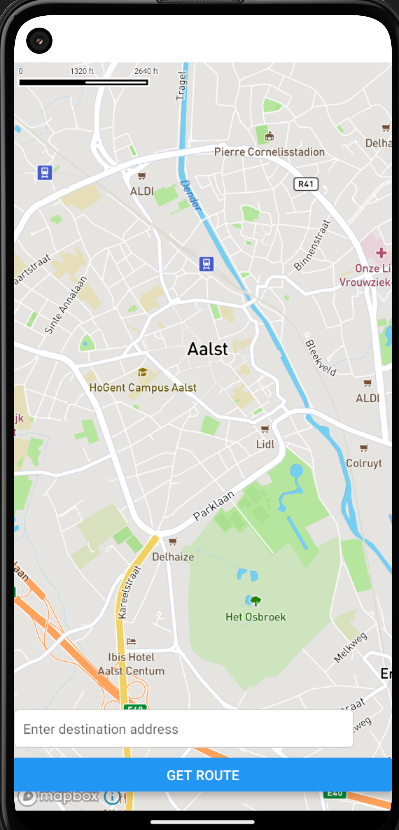
\includegraphics[width=0.5\textwidth]{image.png}
    \caption{Scherm met een knop om de route op te vragen}
    \label{fig:Scherm met een knop om de route op te vragen}
\end{figure}

\begin{figure}[htbp]
    \centering
    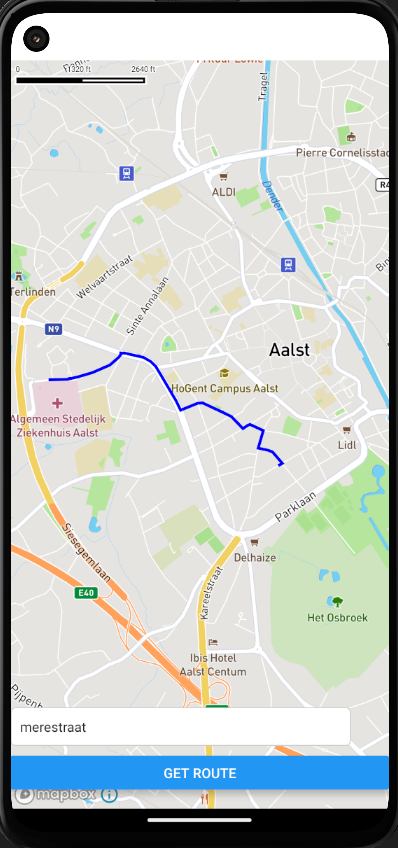
\includegraphics[width=0.5\textwidth]{image-1.png}
    \caption{Scherm met knop waar de route die opgevraagd is}
    \label{fig:Scherm met knop waar route die opgevraagd is}
\end{figure}

\subsection{Installatie en opstarten van de applicatie}
\label{sec:installatie en opstarten van de applicatie}

Zorg ervoor dat Node.js geïnstalleerd is op je systeem en in je \texttt{\$PATH} variabelen staat.
een Mapbox publieke token is nodig om de kaarten te kunnen gebruiken.

\begin{enumerate}
    \item Clone de repository.
    \item Voer `npm install` uit in de hoofdmap van de repository.
    \item In \texttt{App.js}, vervang \texttt{Mapbox.setAccessToken('YOUR\_MAPBOX\_PUBLIC\_KEY');} door je eigen Mapbox publieke token.
    \item Bij \textbf{MapboxUrl} in \texttt{App.js}, vervang \texttt{access\_token=YOUR\_MAPBOX\_PUBLIC\_KEY} aan het einde van de URL met je eigen Mapbox publieke token.
    \item Je hebt ook een \textbf{Google API key} \texttt{YOUR\_GOOGLE\_API\_KEY} nodig voor het maken van de route. Deze kan je verkrijgen op de Google Cloud Platform\footnote{\url{https://cloud.google.com/?hl=nl}}.
    \item Voer `npx expo start` uit om de applicatie te starten. Je kan de optie \texttt{--android} of \texttt{--ios} toevoegen om de applicatie te starten in een specifieke emulator.
    \item Selecteer een emulator of scan de QR code met de Expo app op je telefoon.
\end{enumerate}

\section{Praktijkonderzoek}
\label{sec:praktijkonderzoek}

De proof of concept bevat testen waarbij de requirements ten opzichte van de ontwikkelde applicatie gezet worden en die van Google Maps. Deze testen zullen inzichten, voorkeuren en beperkingen verwerven in wat het beste past bij de doelgroep. In dit deel zal het proces overlopen worden van de testen.

\subsection{Verloop van de testen}
\label{sec:verloop van de testen}

Voor de testen afgenomen worden moet er een duidelijk stappenplan opgesteld worden van hoe de testen uitgevoerd moeten worden. Het belang van deze testen is om te kijken wat het best bij de doelgroep aansluit. Een belangrijk aspect van deze testen is dat de gebruikers hun locatie moeten kunnen onthouden of de locatie vooraf is ingegeven geweest. De eindbestemming kan ook vooraf ingesteld worden voor de doelgroep indien dit een vaste plaats is. \newline

Het testen bestaat uit een paar belangrijke fases. In de voorbereidende fase bepalen waar de gebruiker zich naartoe wil verplaatsen en op welke manier. Ook is het belangrijk dat de applicatie correct staat ingesteld voor de gebruiker.\newline

Het testen van de applicaties zelf zal gebeuren op vlak van verschillende factoren zoals functionaliteiten, de kost en privacy. Hieruit kunnen we dan afstemmen wat het beste pas voor onze doelgroep. Als eerste worden de functionaliteiten getest, welke mogelijkheden zijn er allemaal met de applicatie: de integratie van iconen, de mogelijkheid van AR, offline kaarten, spraakopdrachten, ... . De tweede factor waarmee rekening zal gehouden is de kost. Als laatste is de privacy en gegevensbeheer van de applicatie. Hoe wordt er omgegaan met de gegevens van de gebruiker.

\subsection{Opmerkingen tijdens de testen}
\label{sec:opmerkingen tijdens de testen}

Tijdens het testen vielen enkele zaken op bij het gebruiken van de applicaties. Mapbox is geen `echte` applicatie die je kan installeren. Voor het gebruiken van de Mapbox applicatie moet je een eigen applicatie ontwikkelen voor het gebruiken van hun functionaliteiten. Voor het ontwikkelen van de applicatie is een bepaald vlak van kennis vereist voor deze zaken te kunnen implementeren. De applicatie brengt ook een kost met zich mee er is een gratis level waarop je de API kan gebruiken van Mapbox maar vanaf een bepaald aantal verzoeken is er een pay-as-you-go model waaraan je vasthangt. Naast alle standaard functionaliteiten die Mapbox aanbied zoals een gewone map met een route lijn is de optie van AR mogelijkheid er en het vinden van dichtbij horeca zaken. Ze ondersteunen ook realtime gegevens verkeersinformatie. Op vlak van privacy het enige wat Mapbox vereist is je locatiegegevens indien het gebruik van AR ook je camera. Het grootste voordeel dat Google Maps tov Mapbox biedt is dat het een volledig gratis applicatie waarbij alles functies vrij te verkrijgen zijn waaronder hun AR functie ook wel bekend onder de naam \textit{Live View}. Google Maps biedt ook realtime verkeersinformatie aan en het maakt het mogelijk om route op te slaan voor offline gebruik. Een ander interessant voordeel is dat ze ook de realtime gegevens van het openbaar vervoer bijhouden voor bussen, treinen en trams. Voor privacy vereisen ze dezelfde zaken als die van Mapbox afhankelijk van het gebruik van AR.

%mapbox getest

%google maps getest functies

\section{Discussie}
\label{sec:discussie}

inleiding

\subsection{Resultaten}
\label{sec:resultaten}

vergelijkingen en bemerkingen van de applicaties

\subsection{Alternatief}
\label{sec:alternatief}

Voor mapbox wat kan je doen

\subsection{Reflectie}
\label{sec:reflectie}

Eigen reflectie voor gebruik